% ============================================================
% FENT2321 - Assignment 3
% Preliminary Blade Design and Design-Point Rotor Performance
% ============================================================

\documentclass[11pt,a4paper]{article}

% ------------------------------------------------------------
% Packages
% ------------------------------------------------------------
\usepackage[utf8]{inputenc}
\usepackage[T1]{fontenc}
\usepackage{lmodern}
\usepackage[english]{babel}
\usepackage[a4paper,margin=2.5cm]{geometry}
\usepackage{amsmath,amssymb}
\usepackage{siunitx}
\usepackage{booktabs}
\usepackage{array}
\usepackage{graphicx}
\usepackage{float}
\usepackage{caption}
\usepackage{subcaption}
\usepackage{pgfplots}
\usepackage{pgfplotstable}
\usepackage{xcolor}
\usepackage{enumitem}
\usepackage{hyperref}
\usepackage{microtype}

\pgfplotsset{compat=1.18}

\sisetup{
    per-mode=symbol,
    exponent-product=\cdot,
    output-decimal-marker={.},
    group-separator={,},
    group-minimum-digits=4
}

\hypersetup{
    colorlinks=true,
    linkcolor=black,
    citecolor=black,
    urlcolor=blue,
    pdftitle={Assignment 3 - Preliminary Blade Design}
}

% ------------------------------------------------------------
% Document information
% ------------------------------------------------------------
\title{
    \textbf{FENT2321}\\[0.3cm]
    Wind Energy and Design of a Wind Turbine\\[0.5cm]
    \Large Assignment 3: Preliminary Blade Design and\\
    Design-Point Rotor Performance
}

\author{Markus Arntzen}
\date{}

\begin{document}

\maketitle
\thispagestyle{empty}

\clearpage
\tableofcontents
\clearpage

% ============================================================
\section{Design parameters}
% ============================================================

\begin{table}[H]
\centering
\label{tab:design}
\begin{tabular}{lll}
    \toprule
    Parameter & Value & Unit \\
    \midrule
    Number of blades, $Z$ & 2 & -- \\
    Design wind speed, $V_1$ & 12.0 & \si{m/s} \\
    Design tip-speed ratio, $\lambda_{\mathrm{des}}$ & 4.0 & -- \\
    Rotor radius, $R$ & 0.30 & \si{m} \\
    Number of blade elements, $N$ & 15 & -- \\
    Initial chord at $r/R\approx0.7$ & 50 & \si{mm} \\
    Air density, $\rho$ & 1.2 & \si{kg/m^3} \\
    Dynamic viscosity, $\mu$ & $1.47\times10^{-5}$ & \si{kg/(m\,s)} \\
    Reynolds convergence tolerance & 30000 & -- \\
    Airfoil & NACA 2414 & -- \\
    \bottomrule
\end{tabular}
\caption{Design parameters used for the preliminary blade design.}
\end{table}

The rotational speed corresponding to the design point is

\begin{equation}
    \omega
    =
    \frac{\lambda_{\mathrm{des}}V_1}{R}
    =
    \frac{4.0\cdot12}{0.30}
    =
    \SI{160}{rad/s}.
\end{equation}

% ============================================================
\section{Airfoil selection and aerodynamic data}
% ============================================================

I chose to continue with the NACA 2414NACA. 2414 has a maximum thickness of approximately
14\%, which is consistent with the initial thickness guideline.

The available aerodynamic data used in the calculation are the values of
$C_L$, $C_D$, and $\alpha_{\mathrm{opt}}$ corresponding to the maximum
$C_L/C_D$ at each Reynolds number.

\begin{table}[H]
\centering
\label{tab:polar}
\begin{tabular}{rrrr}
    \toprule
    $Re$ & $C_L$ & $C_D$ & $\alpha_{\mathrm{opt}}$ [deg] \\
    \midrule
    100000  & 0.9155 & 0.01903 & 6.50 \\
    200000  & 0.8850 & 0.01424 & 6.00 \\
    500000  & 0.8155 & 0.01027 & 5.00 \\
    1000000 & 0.8797 & 0.00977 & 5.75 \\
    \bottomrule
\end{tabular}
\caption{NACA 2414 aerodynamic data used in the BEM calculation.}
\end{table}

For Reynolds numbers between the available polar data points, linear
interpolation is used to get accurate values used in the BEM calculations.

% ============================================================
\section{BEM method}
% ============================================================

\subsection{Blade element discretization}

The blade is divided into

\[
    N=15
\]

elements of width

\begin{equation}
    dr=\frac{R}{N}=\frac{0.30}{15}
    =\SI{0.020}{m}.
\end{equation}

The local radius is taken at the centre of each element,

\begin{equation}
    r_i=\left(i-\frac{1}{2}\right)dr,
    \qquad i=1,\ldots,N.
\end{equation}

For $N=15$, one element lies exactly at

\[
    r/R=0.700.
\]

This element is therefore used for the Step 1 and Step 2 Reynolds-number
calculation.

\subsection{Step 1: Initial Reynolds number}

Starting with the assumed values

\[
a=\frac{1}{3},
\qquad
a'=0,
\qquad
c=\SI{0.050}{m}.
\]

At $r/R=0.7$, the relative velocity is

\begin{equation}
W=
\sqrt{
[(1-a)V_1]^2+
[(1+a')\omega r]^2
}.
\end{equation}

The resulting value is approximately

\[
W=\SI{34.54}{m/s}.
\]

The first Reynolds-number estimate is therefore

\begin{equation}
Re_{\mathrm{first}}
=
\frac{\rho Wc}{\mu}
\approx
1.410\times10^5.
\end{equation}

The value used in the calculation is

\[
\boxed{Re_{\mathrm{first}}=140977}.
\]

Since this value lies between $Re=100000$ and $Re=200000$, the corresponding
aerodynamic parameters are obtained by linear interpolation. The resulting
values are approximately

\[
C_L=0.9030,
\qquad
C_D=0.01707,
\qquad
\alpha_{\mathrm{opt}}=6.295^\circ.
\]

\subsection{Step 2: Reynolds-number iteration}

At $r/R=0.7$, the local tip-speed ratio is

\begin{equation}
\lambda_r
=
\frac{r}{R}\lambda_{\mathrm{des}}
=
0.7\cdot4.0
=
2.8.
\end{equation}

The axial induction factor is obtained by solving

\begin{equation}
16a^3-24a^2+a(9-3\lambda_r^2)-1+\lambda_r^2=0.
\end{equation}

The tangential induction factor is

\begin{equation}
a'=\frac{1-3a}{4a-1},
\end{equation}

and the flow angle is

\begin{equation}
\phi
=
\tan^{-1}
\left(
\frac{1-a}{(1+a')\lambda_r}
\right).
\end{equation}

The axial force coefficient is

\begin{equation}
C_a=C_L\cos\phi+C_D\sin\phi.
\end{equation}

The chord is then calculated from

\begin{equation}
\frac{L_c}{R}
=
\frac{
8\pi a(r/R)\sin^2\phi
}{
(1-a)ZC_a
}.
\end{equation}

The relative velocity and new Reynolds number are

\begin{equation}
W=
\sqrt{
[(1-a)V_1]^2+
[(1+a')\omega r]^2
},
\end{equation}

\begin{equation}
Re_{\mathrm{new}}
=
\frac{\rho W L_c}{\mu}.
\end{equation}

The iteration is stopped when

\begin{equation}
\left|Re_{\mathrm{new}}-Re_{\mathrm{old}}\right|
\leq30000.
\end{equation}

The iteration history is shown in Table~\ref{tab:iteration}.

\begin{table}[H]
\centering
\caption{Reynolds-number iteration at $r/R=0.7$.}
\label{tab:iteration}
\begin{tabular}{rrrrrr}
\toprule
Iteration & $Re_{\mathrm{old}}$ & $C_L$ & $C_D$ &
$\alpha_{\mathrm{opt}}$ [deg] & $Re_{\mathrm{new}}$ \\
\midrule
1 & 140977 & 0.90300 & 0.01707 & 6.295 & 219181 \\
2 & 219181 & 0.88056 & 0.01399 & 5.936 & 224925 \\
\bottomrule
\end{tabular}
\end{table}

The second iteration satisfies the convergence criterion because

\[
|224925-219181|
=
5744
<
30000.
\]

The converged Reynolds number is therefore taken as

\[
\boxed{Re=224925}.
\]

Using the converged Reynolds number to interpolate the airfoil data gives

\begin{align}
C_L &= 0.87923,\\
C_D &= 0.01391,\\
\alpha_{\mathrm{des}} &= 5.917^\circ,\\
\frac{C_L}{C_D} &= 63.21.
\end{align}

% ============================================================
\section{Preliminary blade design}
% ============================================================

Once the Reynolds-number iteration has converged, the resulting
$C_L$, $C_D$, and $\alpha_{\mathrm{des}}$ are used for the preliminary blade
design. The local values of $\lambda_r$, $a$, $a'$, $\phi$, and $C_a$ are
calculated separately for every blade element.

The twist angle is calculated as

\begin{equation}
    \theta=\phi-\alpha_{\mathrm{des}}.
\end{equation}

The resulting blade geometry and induction factors are shown in
Table~\ref{tab:geometry}.

\begin{table}[H]
\centering
\caption{Preliminary blade geometry, induction factors, and local Reynolds number.}
\label{tab:geometry}
\small
\begin{tabular}{rrrrrr}
\toprule
$r/R$ & $L_c/R$ & $\theta$ [deg] & $a$ & $a'$ & $Re$ \\
\midrule
0.033 & 0.1983 & 49.020 & 0.2673 & 2.8567 & 52153 \\
0.100 & 0.4201 & 39.549 & 0.2919 & 0.7417 & 122642 \\
0.167 & 0.4873 & 31.623 & 0.3066 & 0.3535 & 162972 \\
0.233 & 0.4812 & 25.400 & 0.3154 & 0.2056 & 186275 \\
0.300 & 0.4482 & 20.620 & 0.3207 & 0.1335 & 200251 \\
0.367 & 0.4088 & 16.941 & 0.3241 & 0.0932 & 209038 \\
0.433 & 0.3709 & 14.071 & 0.3264 & 0.0685 & 214823 \\
0.500 & 0.3370 & 11.793 & 0.3279 & 0.0524 & 218795 \\
0.567 & 0.3073 & 9.954 & 0.3290 & 0.0413 & 221624 \\
0.633 & 0.2817 & 8.444 & 0.3298 & 0.0333 & 223701 \\
0.700 & 0.2595 & 7.186 & 0.3304 & 0.0275 & 225269 \\
0.767 & 0.2402 & 6.123 & 0.3309 & 0.0230 & 226479 \\
0.833 & 0.2234 & 5.216 & 0.3312 & 0.0196 & 227433 \\
0.900 & 0.2087 & 4.432 & 0.3315 & 0.0168 & 228197 \\
0.967 & 0.1956 & 3.750 & 0.3317 & 0.0146 & 228818 \\
\bottomrule
\end{tabular}
\end{table}

The corresponding physical chord lengths range from approximately
\SI{58.7}{mm} at the outermost element to a maximum of approximately
\SI{146.2}{mm} around $r/R=0.167$. To me, this sounds large, but I struggle to
fully understand what I am doing here so it maybe wrong.

% ------------------------------------------------------------
\subsection{Chord distribution}
% ------------------------------------------------------------

Figure~\ref{fig:chord} shows the resulting non-dimensional chord
distribution.

\begin{figure}[H]
\centering
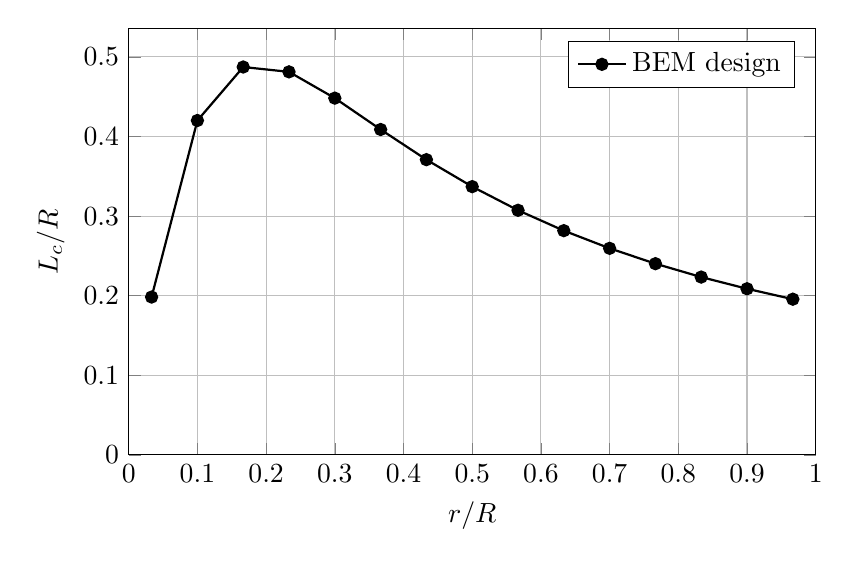
\begin{tikzpicture}
\begin{axis}[
    width=0.85\textwidth,
    height=7cm,
    xlabel={$r/R$},
    ylabel={$L_c/R$},
    grid=both,
    xmin=0,
    xmax=1,
    ymin=0,
    legend pos=north east
]
\addplot[
    mark=*,
    thick
] coordinates {
(0.0333,0.1983)
(0.1000,0.4201)
(0.1667,0.4873)
(0.2333,0.4812)
(0.3000,0.4482)
(0.3667,0.4088)
(0.4333,0.3709)
(0.5000,0.3370)
(0.5667,0.3073)
(0.6333,0.2817)
(0.7000,0.2595)
(0.7667,0.2402)
(0.8333,0.2234)
(0.9000,0.2087)
(0.9667,0.1956)
};
\legend{BEM design}
\end{axis}
\end{tikzpicture}
\caption{Calculated chord distribution along the blade.}
\label{fig:chord}
\end{figure}

\clearpage

% ------------------------------------------------------------
\subsection{Twist distribution}
% ------------------------------------------------------------

Figure~\ref{fig:twist} shows the resulting twist distribution.

\begin{figure}[H]
\centering
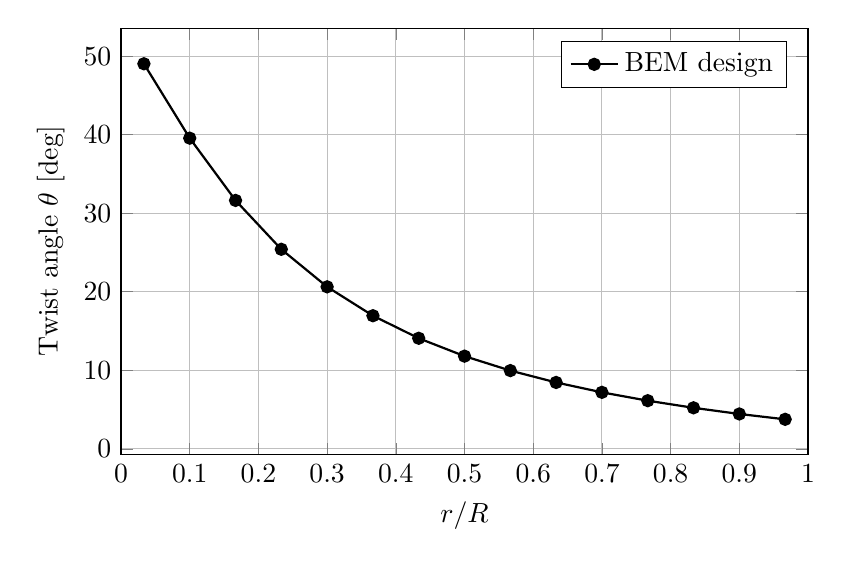
\begin{tikzpicture}
\begin{axis}[
    width=0.85\textwidth,
    height=7cm,
    xlabel={$r/R$},
    ylabel={Twist angle $\theta$ [deg]},
    grid=both,
    xmin=0,
    xmax=1,
    legend pos=north east
]
\addplot[
    mark=*,
    thick
] coordinates {
(0.0333,49.020)
(0.1000,39.549)
(0.1667,31.623)
(0.2333,25.400)
(0.3000,20.620)
(0.3667,16.941)
(0.4333,14.071)
(0.5000,11.793)
(0.5667,9.954)
(0.6333,8.444)
(0.7000,7.186)
(0.7667,6.123)
(0.8333,5.216)
(0.9000,4.432)
(0.9667,3.750)
};
\legend{BEM design}
\end{axis}
\end{tikzpicture}
\caption{Calculated twist distribution along the blade.}
\label{fig:twist}
\end{figure}

% ============================================================
\section{Discussion of blade design}
% ============================================================

\subsection{Induction factors}

The ideal axial induction factor is $a=1/3$ and the ideal tangential
induction factor is $a'=0$. The calculated values approach these ideal
values as the radius increases.

In the outer part of the blade, approximately from $r/R=0.3$ to the tip,
$a$ is between about 0.321 and 0.332. This is close to the ideal value of
$1/3$. The axial induction factor is lower near the root, reaching
approximately $a=0.267$ at the innermost element.

The tangential induction factor shows a much stronger deviation near the
root. It decreases from $a'=2.86$ at $r/R=0.033$ to approximately
$a'=0.0146$ at $r/R=0.967$. It decreases close to zero as we move outwards on the wing.

The large root-region deviations are therefore consistent with the
assignment's warning that the ideal induction factors are mainly expected
over most of the blade rather than at the root.

\subsection{Reynolds-number variation along the blade}

The Reynolds number varies substantially over the blade. The calculated
local value increases from approximately

\[
Re=5.2\times10^4
\]

at the innermost element to

\[
Re=2.29\times10^5
\]

at the outermost element.

At $r/R=0.7$, the local value is approximately

\[
Re=2.25\times10^5,
\]

which is very close to the converged Step 2 value of

\[
Re=2.249\times10^5.
\]

This agreement is expected because Step 2 was specifically performed at
$r/R=0.7$. The Reynolds number is lower than the Step 2 value in the
inboard region and slightly higher toward the tip.

An important limitation is that the innermost calculated Reynolds numbers
fall below the lowest available airfoil polar Reynolds number of $10^5$.
However, Step 3 is prescribed to use the converged aerodynamic parameters
from Step 2 along the blade, so these local Reynolds numbers are reported as
the actual resulting values rather than being used to update the
aerodynamic coefficients.

\subsection{Effect of assuming constant Reynolds number}

The Step 3 design uses the converged aerodynamic parameters from
$r/R\approx0.7$ as representative values along the entire blade. In reality,
the Reynolds number changes from approximately $5.2\times10^4$ near the
root to $2.3\times10^5$ near the tip.

If the aerodynamic coefficients were instead updated locally using the
actual Reynolds number, the chord and twist distributions could change,
particularly in the inboard region where the difference from the
representative Reynolds number is largest. The effect is expected to be
most significant near the root because the local Reynolds number is well
below the Reynolds number used for the Step 2 design. The outer part of the
blade is less affected because its Reynolds number is close to the
converged value.

This is therefore a simplification of the preliminary design procedure.
A locally Reynolds-number-dependent BEM calculation could provide a more
realistic blade design, but this is listed as an optional extension in the
assignment.

\subsection{Comparison with a commercial wind-turbine blade}

The calculated chord distribution has a pronounced inboard region with a
large chord, followed by a gradual reduction in chord toward the tip. This
general tapering behaviour is qualitatively similar to a practical
wind-turbine blade, where the chord normally becomes smaller toward the
tip.

However, the present distribution should not be interpreted as a
manufacturable blade geometry. The chord increases strongly from the first
element to a maximum around $r/R=0.17$, and the root region is governed by
the idealized BEM equations. A commercial blade would normally have a
structurally designed root, a smoother transition from the root section,
and additional practical constraints. The assignment explicitly treats
the hub as visualization only at this stage, and production constraints are
handled later in Assignment 4.

Thus, the present chord distribution captures the aerodynamic tapering
trend but should be regarded as a preliminary aerodynamic design rather
than a final commercial blade geometry.

% ============================================================
\section{Forces acting on the blade}
% ============================================================

For each blade element, the normal and tangential force coefficients are
calculated from

\begin{align}
C_n &= C_L\cos\phi+C_D\sin\phi,\\
C_t &= C_L\sin\phi-C_D\cos\phi.
\end{align}

The element thrust and tangential force for all $Z$ blades are calculated
using

\begin{align}
Z\,dT'
&=
Z\left(
\frac{1}{2}\rho W^2 c C_n\,dr
\right),\\
Z\,dM'
&=
Z\left(
\frac{1}{2}\rho W^2 c C_t\,dr
\right).
\end{align}

The torque contribution from each element is

\begin{equation}
dQ=r(Z\,dM').
\end{equation}

The calculated force distribution is given in
Table~\ref{tab:forces}.

\begin{table}[H]
\centering
\caption{Thrust and tangential force acting on all two blades for each blade element.}
\label{tab:forces}
\small
\begin{tabular}{rrr}
\toprule
$r/R$ & $Z\,dT'$ [N] & $Z\,dM'$ [N] \\
\midrule
0.033 & 0.085 & 0.117 \\
0.100 & 0.269 & 0.265 \\
0.167 & 0.462 & 0.343 \\
0.233 & 0.656 & 0.385 \\
0.300 & 0.852 & 0.409 \\
0.367 & 1.047 & 0.422 \\
0.433 & 1.241 & 0.429 \\
0.500 & 1.436 & 0.434 \\
0.567 & 1.630 & 0.436 \\
0.633 & 1.824 & 0.436 \\
0.700 & 2.018 & 0.436 \\
0.767 & 2.211 & 0.435 \\
0.833 & 2.405 & 0.434 \\
0.900 & 2.599 & 0.432 \\
0.967 & 2.792 & 0.430 \\
\bottomrule
\end{tabular}
\end{table}

The thrust force increases toward the blade tip because the local relative
velocity increases strongly with radius. The tangential force reaches a
fairly broad maximum in the mid-to-outer part of the blade and then changes
only slightly toward the tip.

% ============================================================
\section{Design-point rotor performance}
% ============================================================

The total rotor thrust and torque are obtained by summing the blade-element
contributions:

\begin{align}
T &= \sum_i Z\,dT'_i,\\
Q &= \sum_i r_i(Z\,dM'_i).
\end{align}

The total power is

\begin{equation}
P=\omega Q.
\end{equation}

The power and thrust coefficients are calculated from

\begin{align}
C_P &=
\frac{P}
{\frac{1}{2}\rho A V_1^3},\\
C_T &=
\frac{T}
{\frac{1}{2}\rho A V_1^2},
\end{align}

where

\[
A=\pi R^2.
\]

The resulting design-point performance is

\begin{table}[H]
\centering
\caption{Design-point rotor performance.}
\label{tab:performance}
\begin{tabular}{lrl}
\toprule
Quantity & Value & Unit \\
\midrule
Total thrust, $T$ & 21.526 & N \\
Total torque, $Q$ & 0.9559 & N\,m \\
Power, $P$ & 152.94 & W \\
Power coefficient, $C_P$ & 0.5217 & -- \\
Thrust coefficient, $C_T$ & 0.8812 & -- \\
\bottomrule
\end{tabular}
\end{table}

\end{document}